% answers.tex —— 2000 年·春季京皖卷·理科 · 参考答案与详细解析片段
% 由 tools/generate_projects.py 依来源总账自 2000/2000_数学真题_春季京皖理_试题.md + 2000/2000_数学真题_春季京皖理_解析正文.md + 2000/2000_数学真题_春季京皖理_答案要点.md 生成，勿手改（改源 MD 后重跑）


\begin{gknotice}
\textbf{解析归属}：固定源 PDF 只有题面，没有答案页。以下推导依据固定题面形成，\textbf{非官方解析}；已由独立解题者在只读题面条件下盲解（24 题），转录另经 300 dpi 与内容流核对。源内疑点保留在题面与答案要点中，不以推导结果反改原题。
\end{gknotice}

\begin{answer}
\gksolhead{1}{}

\textbf{题目}：

复数 $z_1 = 3 + \mathrm{i}$，$z_2 = 1 - \mathrm{i}$，则 $z = z_1 \cdot z_2$ 在复平面内的对应点位于　（　）

（A）第一象限　（B）第二象限　（C）第三象限　（D）第四象限

\Needspace{4\baselineskip}
\textbf{解析}

$z=z_1z_2=(3+\mathrm i)(1-\mathrm i)=3-3\mathrm i+\mathrm i-\mathrm i^2=4-2\mathrm i$，对应点 $(4,-2)$，实部为正、虚部为负，位于第四象限。

验证：按 $(a+b\mathrm i)(c+d\mathrm i)=(ac-bd)+(ad+bc)\mathrm i$ 复核：实部 $3\cdot1-1\cdot(-1)=4$，虚部 $3\cdot(-1)+1\cdot1=-2$，与直接展开一致；点 $(4,-2)$ 在第四象限。

\gkanswer{答案：D}

\par\medskip

\end{answer}
\begin{answer}
\gksolhead{2}{}

\textbf{题目}：

设全集 $I = \{a, b, c, d, e\}$，集合 $M = \{a, c, d\}$，$N = \{b, d, e\}$，那么 $\overline{M} \cap \overline{N}$ 是　（　）

（A）$\varnothing$　（B）$\{d\}$　（C）$\{a, c\}$　（D）$\{b, e\}$

\Needspace{4\baselineskip}
\textbf{解析}

\Needspace{5\baselineskip}
$I=\{a,b,c,d,e\}$，$M=\{a,c,d\}$，$N=\{b,d,e\}$，于是 $\complement_I M=\{b,e\}$，$\complement_I N=\{a,c\}$，

\nopagebreak[4]
\[\overline M\cap\overline N=\{b,e\}\cap\{a,c\}=\varnothing .\]

（也可用德摩根律：$\overline M\cap\overline N=\complement_I(M\cup N)$，而 $M\cup N=I$。）

验证：逐元素核对 $I$ 的五个元素：$a\in M$，$b\in N$，$c\in M$，$d\in M\cap N$，$e\in N$；没有一个元素同时落在两个补集中，故交集为空集。

\gkanswer{答案：A}

\par\medskip

\end{answer}
\begin{answer}
\gksolhead{3}{}

\textbf{题目}：

已知双曲线 $\frac{x^2}{b^2} - \frac{y^2}{a^2} = 1$ 的两条渐近线互相垂直，那么该双曲线的离心率是　（　）

（A）$2$　（B）$\sqrt{3}$　（C）$\sqrt{2}$　（D）$\frac{3}{2}$

\Needspace{4\baselineskip}
\textbf{解析}

\Needspace{5\baselineskip}
双曲线 $\dfrac{x^2}{b^2}-\dfrac{y^2}{a^2}=1$ 的渐近线为 $y=\pm\dfrac{a}{b}x$。两渐近线互相垂直：

\nopagebreak[4]
\[\frac{a}{b}\cdot\left(-\frac{a}{b}\right)=-1\ \Longrightarrow\ a^2=b^2 .\]

实半轴为 $b$，故 $c^2=a^2+b^2=2b^2$，$e=\dfrac{c}{b}=\sqrt2$。

验证：取 $a=b=1$，渐近线 $y=\pm x$ 确为互相垂直，$c=\sqrt2$，$e=\sqrt2$；若 $a\ne b$（如 $a=1,b=2$），斜率之积为 $-\tfrac14\ne-1$，不垂直，故 $a=b$ 是唯一可能。

\gkanswer{答案：C}

\par\medskip

\end{answer}
\begin{answer}
\gksolhead{4}{}

\textbf{题目}：

曲线 $xy = 1$ 的参数方程是　（　）

（A）$\begin{cases} x = t^{\frac{1}{2}}, \\ y = t^{-\frac{1}{2}}. \end{cases}$　（B）$\begin{cases} x = \sin\alpha, \\ y = \csc\alpha. \end{cases}$

（C）$\begin{cases} x = \cos\alpha, \\ y = \sec\alpha. \end{cases}$　（D）$\begin{cases} x = \tan\alpha, \\ y = \cot\alpha. \end{cases}$

\Needspace{4\baselineskip}
\textbf{解析}

四个选项在各自有定义处都满足 $xy=1$，区别在于参数方程能否\textbf{恰好表示整条曲线}：

\begin{itemize}
\item (A) $x=t^{1/2}>0,\ y=t^{-1/2}>0\ (t>0)$：只覆盖第一象限的一支；
\item (B) $x=\sin\alpha\in[-1,1]\setminus\{0\},\ y=\csc\alpha$：只覆盖 $|x|\le1$ 的部分；
\item (C) $x=\cos\alpha\in[-1,1]\setminus\{0\},\ y=\sec\alpha$：同样只覆盖 $|x|\le1$；
\item (D) $x=\tan\alpha$ 取遍 $\mathbb R\setminus\{0\}$，$y=\cot\alpha=\dfrac1x$：覆盖 $xy=1$ 的全部点。
\end{itemize}

故只有 (D) 是曲线 $xy=1$ 的参数方程。

验证：曲线上的点 $\left(2,\tfrac12\right)$ 由 $\alpha=\arctan 2$ 代入 (D) 可得；(B)(C) 均无法取到 $x=2$；(A) 虽可取 $t=4$ 得到该点，却无法表示第三象限的点 $(-2,-\tfrac12)$。因此只有 (D) 表示整条曲线。

注：四个选项代回都满足 $xy=1$，按参数方程的定义（图像与曲线重合）判定，取 (D)。

\gkanswer{答案：D}

\par\medskip

\end{answer}
\begin{answer}
\gksolhead{5}{}

\textbf{题目}：

一个圆锥的底面直径和高都同一个球的直径相等，那么圆锥与球的体积之比是　（　）

（A）$1:3$　（B）$2:3$　（C）$1:2$　（D）$2:9$

\Needspace{4\baselineskip}
\textbf{解析}

\Needspace{5\baselineskip}
设球半径为 $R$，直径为 $2R$。圆锥底面直径 $=2R$，故底面半径 $R$、高 $2R$：

\nopagebreak[4]
\[V_{\text{\text{锥}}}=\frac13\pi R^2\cdot 2R=\frac{2\pi R^3}{3},\qquad V_{\text{\text{球}}}=\frac43\pi R^3,\]

\nopagebreak[4]
\[\frac{V_{\text{\text{锥}}}}{V_{\text{\text{球}}}}=\frac{2}{4}=\frac12 .\]

验证：取 $R=1$：$V_{\text{\text{锥}}}=\tfrac{2\pi}{3}\approx2.094$，$V_{\text{\text{球}}}=\tfrac{4\pi}{3}\approx4.189$，比值为 $1:2$。

\gkanswer{答案：C}

\par\medskip

\end{answer}
\begin{answer}
\gksolhead{6}{}

\textbf{题目}：

直线 $\theta = a$ 和直线 $\rho\sin(\theta - a) = 1$ 的位置关系是　（　）

（A）垂直　（B）平行　（C）相交但不垂直　（D）重合

\Needspace{4\baselineskip}
\textbf{解析}

\Needspace{5\baselineskip}
$\theta=a$ 是过极点、方向向量为 $(\cos a,\sin a)$ 的直线。由 $\rho\sin(\theta-a)=1$ 得

\nopagebreak[4]
\[\rho(\sin\theta\cos a-\cos\theta\sin a)=1\ \Longrightarrow\ -x\sin a+y\cos a=1 ,\]

其法向量 $\mathbf n=(-\sin a,\cos a)$ 与 $\theta=a$ 的方向向量 $(\cos a,\sin a)$ 内积为 $-\sin a\cos a+\cos a\sin a=0$，故该法向量垂直于第一条直线的方向，即两直线平行；又第二条直线不过极点（原点代入左端为 $0\ne1$），故不重合。

验证：取 $a=0$：两直线分别为 $x$ 轴与 $y=1$，确实平行且不重合。

\gkanswer{答案：B}

\par\medskip

\end{answer}
\begin{answer}
\gksolhead{7}{}

\textbf{题目}：

函数 $y = \lg |x|$　（　）

（A）是偶函数，在区间 $(-\infty, 0)$ 上单调递增

（B）是偶函数，在区间 $(-\infty, 0)$ 上单调递减

（C）是奇函数，在区间 $(0, +\infty)$ 上单调递增

（D）是奇函数，在区间 $(0, +\infty)$ 上单调递减

\Needspace{4\baselineskip}
\textbf{解析}

$f(-x)=\lg|-x|=\lg|x|=f(x)$，故为偶函数。当 $x<0$ 时 $f(x)=\lg(-x)$，而 $y=-x$ 在 $(-\infty,0)$ 上递减、$\lg$ 递增，复合后 $f$ 在 $(-\infty,0)$ 上单调递减。

验证：$f(-4)=\lg4\approx0.602$，$f(-2)=\lg2\approx0.301$：$x$ 由 $-4$ 增大到 $-2$ 时函数值减小，确为递减。

\gkanswer{答案：B}

\par\medskip

\end{answer}
\begin{answer}
\gksolhead{8}{}

\textbf{题目}：

从单词“equation”选取 5 个不同的字母排成一排，含有“qu”（其中“qu”相连且顺序不变）的不同排列共有　（　）

（A）120 个　（B）480 个　（C）720 个　（D）840 个

\Needspace{4\baselineskip}
\textbf{解析}

\Needspace{5\baselineskip}
「equation」的字母 $e,q,u,a,t,i,o,n$ 共 8 个且互不相同。把「$qu$」捆绑成一个整体，再从其余 6 个字母中选 3 个，与整体一起全排列：

\nopagebreak[4]
\[\mathrm C_6^3\cdot 4!=20\times24=480 .\]

验证：换一种数法：先定「$qu$」在 4 个位置中的位置（4 种），再将其余 3 个字母按顺序填入剩余 3 个位置：$4\times \mathrm A_6^3=4\times120=480$，与上一致。

\gkanswer{答案：B}

\par\medskip

\end{answer}
\begin{answer}
\gksolhead{9}{}

\textbf{题目}：

椭圆短轴长是 2，长轴长是短轴的 2 倍，则椭圆中心到其准线距离是　（　）

（A）$\frac{8}{5}\sqrt{5}$　（B）$\frac{4}{5}\sqrt{5}$　（C）$\frac{8}{3}\sqrt{3}$　（D）$\frac{4}{3}\sqrt{3}$

\Needspace{4\baselineskip}
\textbf{解析}

\Needspace{5\baselineskip}
短轴长 $2b=2\Rightarrow b=1$；长轴长是短轴的 2 倍，即 $2a=2\times2\Rightarrow a=2$；$c=\sqrt{a^2-b^2}=\sqrt3$。椭圆中心到准线的距离为

\nopagebreak[4]
\[\frac{a^2}{c}=\frac{4}{\sqrt3}=\frac{4\sqrt3}{3}.\]

验证：准线 $x=\pm\dfrac{4\sqrt3}{3}\approx\pm2.309$，满足准线在椭圆外（$|x|>a=2$），数值合理。

\gkanswer{答案：D}

\par\medskip

\end{answer}
\begin{answer}
\gksolhead{10}{}

\textbf{题目}：

函数 $y = \dfrac{1}{2 + \sin x + \cos x}$ 的最大值是　（　）

（A）$\dfrac{\sqrt{2}}{2} - 1$　（B）$\dfrac{\sqrt{2}}{2} + 1$　（C）$1 - \dfrac{\sqrt{2}}{2}$　（D）$-1 - \dfrac{\sqrt{2}}{2}$

\Needspace{4\baselineskip}
\textbf{解析}

\Needspace{5\baselineskip}
$\sin x+\cos x=\sqrt2\sin\!\left(x+\dfrac\pi4\right)\in[-\sqrt2,\sqrt2]$，故分母最小为 $2-\sqrt2>0$，于是

\nopagebreak[4]
\[y_{\max}=\frac{1}{2-\sqrt2}=\frac{2+\sqrt2}{4-2}=1+\frac{\sqrt2}{2}.\]

验证：取 $x=\dfrac{5\pi}{4}$：$\sin x+\cos x=-\sqrt2$，$y=\dfrac{1}{2-\sqrt2}\approx1.707$ 为最大；取 $x=\dfrac{\pi}{4}$：$y=\dfrac{1}{2+\sqrt2}\approx0.293$ 为最小，与「分母最小则 $y$ 最大」一致。

\gkanswer{答案：B}

\par\medskip

\end{answer}
\begin{answer}
\gksolhead{11}{}

\textbf{题目}：

设复数 $z_1 = 2\sin\theta + \mathrm{i}\cos\theta$（$\frac{\pi}{4} < \theta < \frac{\pi}{2}$）在复平面上对应向量 $\overrightarrow{OZ_1}$，将 $\overrightarrow{OZ_1}$ 按顺时针方向旋转 $\frac{3}{4}\pi$ 后得到向量 $\overrightarrow{OZ_2}$，$\overrightarrow{OZ_2}$ 对应的复数为 $z_2 = r(\cos\varphi + \mathrm{i}\sin\varphi)$，则 $\tan\varphi =$　（　）

（A）$\frac{2\tan\theta + 1}{2\tan\theta - 1}$　（B）$\frac{2\tan\theta - 1}{2\tan\theta + 1}$　（C）$\frac{1}{2\tan\theta + 1}$　（D）$\frac{1}{2\tan\theta - 1}$

\Needspace{4\baselineskip}
\textbf{解析}

\Needspace{5\baselineskip}
顺时针旋转 $\dfrac{3\pi}{4}$ 即乘以 $\mathrm e^{-\mathrm i\frac{3\pi}{4}}=-\dfrac{\sqrt2}{2}(1+\mathrm i)$。于是

\nopagebreak[4]
\[\begin{aligned}
z_2&=-\frac{\sqrt2}{2}\,(2\sin\theta+\mathrm i\cos\theta)(1+\mathrm i)\\
&=-\frac{\sqrt2}{2}\Big[(2\sin\theta-\cos\theta)+\mathrm i(2\sin\theta+\cos\theta)\Big].
\end{aligned}\]

\Needspace{5\baselineskip}
故

\nopagebreak[4]
\[\tan\varphi=\frac{\operatorname{Im}z_2}{\operatorname{Re}z_2}=\frac{2\sin\theta+\cos\theta}{2\sin\theta-\cos\theta}=\frac{2\tan\theta+1}{2\tan\theta-1},\]

其中 $\theta\in\left(\dfrac\pi4,\dfrac\pi2\right)$ 保证 $\cos\theta>0$、$2\tan\theta-1>0$，约分合法。

验证：取 $\theta=\dfrac\pi3$：$z_1=\sqrt3+\tfrac12\mathrm i$，旋转后 $z_2$ 的实部 $\approx-0.871$、虚部 $\approx-1.578$，$\tan\varphi\approx1.812$；公式给出 $\dfrac{2\sqrt3+1}{2\sqrt3-1}=\dfrac{4.464}{2.464}\approx1.812$，一致。

\gkanswer{答案：A}

\par\medskip

\end{answer}
\begin{answer}
\gksolhead{12}{}

\textbf{题目}：

设 $\alpha$，$\beta$ 是一个钝角三角形的两个锐角，下列四个不等式中不正确的是　（　）

（A）$\tan\alpha\tan\beta < 1$　（B）$\sin\alpha + \sin\beta < \sqrt{2}$

（C）$\cos\alpha + \cos\beta > 1$　（D）$\frac{1}{2}\tan(\alpha+\beta) < \tan\frac{\alpha+\beta}{2}$

\Needspace{4\baselineskip}
\textbf{解析}

钝角三角形的两个锐角满足 $\alpha+\beta<90^\circ$，逐项判断：

\begin{itemize}
\item (A) $\tan(\alpha+\beta)=\dfrac{\tan\alpha+\tan\beta}{1-\tan\alpha\tan\beta}>0$，而分子 $>0$，故分母 $1-\tan\alpha\tan\beta>0$，即 $\tan\alpha\tan\beta<1$，正确；
\item (B) $\beta<90^\circ-\alpha\Rightarrow\sin\beta<\cos\alpha$，故 $\sin\alpha+\sin\beta<\sin\alpha+\cos\alpha\le\sqrt2$（后一等号仅在 $\alpha=45^\circ$ 时取到，但此时 $\beta<45^\circ$ 使前式严格），正确；
\item (C) $\beta<90^\circ-\alpha\Rightarrow\cos\beta>\cos(90^\circ-\alpha)=\sin\alpha$，故 $\cos\alpha+\cos\beta>\cos\alpha+\sin\alpha\ge1$，正确；
\item (D) 记 $s=\alpha+\beta\in(0^\circ,90^\circ)$，$t=\tan\dfrac s2\in(0,1)$，则 $\dfrac12\tan s=\dfrac{t}{1-t^2}>t=\tan\dfrac s2$，故 (D) 的不等号方向反了，\textbf{不正确}。
\end{itemize}

验证：取 $\alpha=\beta=30^\circ$：(A) $\tfrac13<1$、(B) $1<\sqrt2$、(C) $\sqrt3>1$ 均成立；而 (D) 左端 $\tfrac12\tan60^\circ\approx0.866$，右端 $\tan30^\circ\approx0.577$，$0.866<0.577$ 不成立。故选 D。

\gkanswer{答案：D}

\par\medskip

\end{answer}
\begin{answer}
\gksolhead{13}{}

\textbf{题目}：

已知等差数列 $\{a_n\}$ 满足 $a_1 + a_2 + a_3 + \cdots + a_{101} = 0$，则有　（　）

（A）$a_1 + a_{101} > 0$　（B）$a_2 + a_{100} < 0$　（C）$a_3 + a_{99} = 0$　（D）$a_{51} = 51$

\Needspace{4\baselineskip}
\textbf{解析}

\Needspace{5\baselineskip}
等差数列前 101 项和 $S_{101}=\dfrac{101(a_1+a_{101})}{2}=101a_{51}=0$，故 $a_{51}=0$。于是

\nopagebreak[4]
\[a_3+a_{99}=2a_{51}=0 .\]

验证：取常数列 $a_n\equiv0$（满足条件），可排除 (A)(B)(D)：$a_1+a_{101}=0$ 不 $>0$，$a_2+a_{100}=0$ 不 $<0$，$a_{51}=0\ne51$；而 $a_3+a_{99}=0$ 成立。

\gkanswer{答案：C}

\par\medskip

\end{answer}
\begin{answer}
\gksolhead{14}{}

\textbf{题目}：

已知函数 $f(x) = ax^3 + bx^2 + cx + d$ 的图象如图，则　（　）
\nopagebreak[4]
\begin{center}% f2000_spring_jingwan_science_q14_graph.tex — 2000 年·春季京皖卷·理科 第 14 题（f(x)=ax³+bx²+cx+d 的图象）
%
% 【来源】`.work/phase4-b20/source/2000春季京皖理.pdf`
%   （SHA-256 37f07244497aa0a21be12d8a31eac78b61490f835f088719a5990463585a35ce），
%   第 1 页（印刷页 61）；qpdf --qdf 解包后对内容流逐路径解析。
% 【坐标口径】源 PDF 用户空间（原点左下、y 向上）。本图本地坐标
%   (x, y) = (x_page − 608.528, y_page − 518.047)，1 单位 = 1 TeX pt；
%   O 取两轴交点；x 轴 y_page ≡ 518.047，y 轴 x_page ≡ 608.528。
% 【元素计数】5 条路径（x 轴／x 箭头／y 轴／y 箭头／曲线）＋ 5 个标签。
% 【标签】位置取 pdftotext -bbox 文本中心换算（源中心逐条记在 \node 行末）；
%   本图有 3 处微调（源位与微调量见各 \node 行末）：「O」左移 2.2 pt 避曲线，
%   「1」「2」同步下移 2.56 pt（保持两刻度同基线；「2」原净距仅 1.0 pt）。
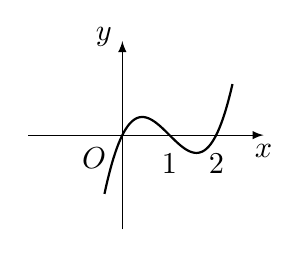
\begin{tikzpicture}[x=1pt, y=1pt,
    every node/.style={inner sep=0pt, font=\fontsize{10.5pt}{12.6pt}\selectfont}]
  \draw[line width=0.399pt] (-34.017,0) -- (47.438,0);
  \fill[line width=0.399pt] (51.025,0) .. controls (49.962,0.199) and (48.235,0.797) .. (47.04,1.494) -- (47.04,-1.494) .. controls (48.235,-0.797) and (49.962,-0.199) .. (51.025,0);
  \draw[line width=0.399pt] (0,-34.017) -- (0,30.43);
  \fill[line width=1.000pt] (0,34.016) .. controls (-0.199,32.954) and (-0.797,31.227) .. (-1.494,30.031) -- (1.494,30.031) .. controls (0.797,31.227) and (0.199,32.954) .. (0,34.016);
  % 曲线（本图第 5 条路径）：7177 个采样点 / 299 段三次贝塞尔。最小二乘拟合
  %   y = 0.003457x^3 - 0.176384x^2 + 1.999983x（rms 0.0002 pt，最大偏差 0.0025 pt），按该式绘制。
  \draw[line width=0.797pt, domain=-6.4632:39.7852, samples=240]
    plot (\x, {0.003457*\x*\x*\x - 0.176384*\x*\x + 1.999983*\x});

  \node[anchor=center] at (-6.648,35.403) {$y$};  % 源中心 (601.88,553.45)
  \node[anchor=center] at (-10.198,-8.247) {$O$};  % 源中心 (600.53,509.80)；左移 2.2 pt 避曲线（原净距 1.0 pt）
  \node[anchor=center] at (17.012,-10.397) {$1$};  % 源中心 (625.54,510.21)；与 2 同步下移 2.56 pt 保持同基线
  \node[anchor=center] at (34.012,-10.397) {$2$};  % 源中心 (642.54,510.21)；下移 2.56 pt 避曲线（原净距 1.0 pt）
  \node[anchor=center] at (51.022,-5.597) {$x$};  % 源中心 (659.55,512.45)
\end{tikzpicture}
%
% 【自验】
%   1) 探针编译：/tmp 最小文档（ctexart + common/preamble + xelatex）\input 本文件，0 error、0 warning。
%   2) 600 dpi 双渲染差分（有标签 / 标签 opacity=0）量测标签墨迹到路径墨迹最近距离：
%      各标签净距：「2」2.80、「x」2.85、「O」3.06、「1」4.35、「y」5.24 —— 最小 2.80 pt。
%   3) 线形：两轴 0.399 pt，曲线 0.797 pt，实线，与源 w 值一致；箭头为源贝塞尔填充路径。
%   4) 曲线拟合残差 rms 0.0002 pt、最大 0.0025 pt；根 x=0、17.00、34.02 与源标注 1、2 对位。
\end{center}
\nopagebreak[4]
（A）$b \in (-\infty, 0)$　（B）$b \in (0, 1)$　（C）$b \in (1, 2)$　（D）$b \in (2, +\infty)$

\Needspace{4\baselineskip}
\textbf{解析}

\Needspace{5\baselineskip}
由图象：曲线过原点，且与 $x$ 轴另交于 $x=1$、$x=2$；右端上升，故三次项系数 $a>0$。于是

\nopagebreak[4]
\[f(x)=a\,x(x-1)(x-2)=a\big(x^3-3x^2+2x\big),\]

比较系数得 $b=-3a<0$，即 $b\in(-\infty,0)$。

验证：$f'(x)=a(3x^2-6x+2)$ 的零点为 $1\pm\dfrac{\sqrt3}{3}\approx0.42,\ 1.58$，恰与图中「极大点在 $(0,1)$ 内、极小点在 $(1,2)$ 内」吻合。另：即使把图中 1、2 误读为极值点，也有 $b=-\dfrac92a<0$，结论不变。

\gkanswer{答案：A}

\par\medskip

\end{answer}
\begin{answer}
\gksolhead{15}{}

\textbf{题目}：

函数 $y = \cos\left(\frac{2\pi}{3}x + \frac{\pi}{4}\right)$ 的最小正周期是\gkblank{}．

\Needspace{4\baselineskip}
\textbf{解析}

\Needspace{5\baselineskip}
$y=\cos\!\left(\dfrac{2\pi}{3}x+\dfrac\pi4\right)$ 的周期

\nopagebreak[4]
\[T=\frac{2\pi}{\,2\pi/3\,}=3 .\]

验证：$\cos\!\left[\dfrac{2\pi}{3}(x+3)+\dfrac\pi4\right]=\cos\!\left(\dfrac{2\pi}{3}x+\dfrac\pi4+2\pi\right)$，函数值不变，故 3 是周期；且 $3$ 为最小正周期（$\omega=\tfrac{2\pi}{3}$）。

\gkanswer{答案：$3$}

\par\medskip

\end{answer}
\begin{answer}
\gksolhead{16}{}

\textbf{题目}：

已知一体积为 72 的正四面体，连结两个面的重心 $E$、$F$，则线段 $EF$ 的长是\gkblank{}．

\Needspace{4\baselineskip}
\textbf{解析}

\Needspace{5\baselineskip}
设正四面体棱长为 $a$，体积 $V=\dfrac{\sqrt2}{12}a^3=72$，故

\nopagebreak[4]
\[a^3=432\sqrt2=(6\sqrt2)^3\ \Longrightarrow\ a=6\sqrt2 .\]

\Needspace{5\baselineskip}
正四面体四个面的重心构成一个棱长为 $\dfrac a3$ 的正四面体（任取两面，其重心连线平行于公共棱的对棱且长度为该对棱的 $\dfrac13$），故

\nopagebreak[4]
\[EF=\frac a3=2\sqrt2 .\]

验证：代回体积：$\dfrac{\sqrt2}{12}(6\sqrt2)^3=\dfrac{\sqrt2}{12}\cdot432\sqrt2=72$，与题设一致；坐标法取棱长 1 时两面重心距离为 $\tfrac13$，比例正确。

\gkanswer{答案：$2\sqrt2$}

\par\medskip

\end{answer}
\begin{answer}
\gksolhead{17}{}

\textbf{题目}：

$\left(\sqrt{x} - \frac{1}{\sqrt[3]{x}}\right)^{10}$ 展开式中的常数项是\gkblank{}．

\Needspace{4\baselineskip}
\textbf{解析}

\Needspace{5\baselineskip}
通项

\nopagebreak[4]
\[\mathrm T_{k+1}=\mathrm C_{10}^k(\sqrt x)^{10-k}\left(-\frac{1}{\sqrt[3]x}\right)^{k}=\mathrm C_{10}^k(-1)^k x^{\frac{10-k}{2}-\frac k3}.\]

\Needspace{5\baselineskip}
令指数为零：$\dfrac{10-k}{2}-\dfrac k3=0\Rightarrow3(10-k)=2k\Rightarrow k=6$。故常数项为

\nopagebreak[4]
\[\mathrm C_{10}^6(-1)^6=210 .\]

验证：$k=6$ 时指数 $\dfrac{10-6}{2}-\dfrac63=2-2=0$，确为常数项；$\mathrm C_{10}^6=\mathrm C_{10}^4=210$。

\gkanswer{答案：$210$}

\par\medskip

\end{answer}
\begin{answer}
\gksolhead{18}{}

\textbf{题目}：

在空间，下列命题正确的是\gkblank{}．（注：把你认为正确的命题的序号都填上）

① 如果两直线 $a$、$b$ 分别与直线 $l$ 平行，那么 $a \parallel b$；

② 如果直线 $a$ 与平面 $\beta$ 内的一条直线 $b$ 平行，那么 $a \parallel \beta$；

③ 如果直线 $a$ 与平面 $\beta$ 内的两条直线 $b$、$c$ 都有垂直，那么 $a \perp \beta$；

④ 如果平面 $\beta$ 内的一条直线 $a$ 垂直平面 $\gamma$，那么 $\beta \perp \gamma$．

\Needspace{4\baselineskip}
\textbf{解析}

\begin{itemize}
\item ① 平行于同一直线的两条直线平行（公理 4），\textbf{正确}；
\item ② 直线 $a$ 可能与平面 $\beta$ 内直线 $b$ 平行却 $a\subset\beta$，此时 $a\not\parallel\beta$，\textbf{错误}；
\item ③ 需 $b,c$ \textbf{相交}；若 $b\parallel c$，则不能判定 $a\perp\beta$，\textbf{错误}；
\item ④ 由线面垂直的性质与面面垂直的判定定理，$a\subset\beta$ 且 $a\perp\gamma\Rightarrow\beta\perp\gamma$，\textbf{正确}。
\end{itemize}

验证：反例：②取 $a\subset\beta$ 且 $a\parallel b$；③取 $b\parallel c$ 时 $a$ 可在 $\beta$ 内斜交。①④为定理，无反例。

\gkanswer{答案：①④}

\par\medskip

\end{answer}
\begin{answer}
\gksolhead{19}{}

\textbf{题目}：

在 $\triangle ABC$ 中，角 $A$、$B$、$C$ 对边分别为 $a$、$b$、$c$，证明：$\dfrac{a^2 - b^2}{c^2} = \dfrac{\sin(A - B)}{\sin C}$．

\Needspace{4\baselineskip}
\textbf{解析}

\Needspace{5\baselineskip}
由正弦定理 $\dfrac{a}{\sin A}=\dfrac{b}{\sin B}=\dfrac{c}{\sin C}=2R$，得 $a=2R\sin A$，$b=2R\sin B$，$c=2R\sin C$。于是

\nopagebreak[4]
\[\frac{a^2-b^2}{c^2}=\frac{\sin^2A-\sin^2B}{\sin^2C}.\]

\Needspace{5\baselineskip}
由恒等式 $\sin^2A-\sin^2B=\sin(A+B)\sin(A-B)$，并注意 $A+B=\pi-C$，得

\nopagebreak[4]
\[\sin^2A-\sin^2B=\sin C\,\sin(A-B).\]

\Needspace{5\baselineskip}
代入即得

\nopagebreak[4]
\[\frac{a^2-b^2}{c^2}=\frac{\sin C\sin(A-B)}{\sin^2C}=\frac{\sin(A-B)}{\sin C}. \qquad\blacksquare\]

验证：取 $A=60^\circ,B=30^\circ,C=90^\circ$（对应 $a:b:c=\sin60^\circ:\sin30^\circ:1$）：左端 $\dfrac{\sin^260^\circ-\sin^230^\circ}{\sin^290^\circ}=\dfrac34-\dfrac14=\dfrac12$；右端 $\dfrac{\sin30^\circ}{\sin90^\circ}=\dfrac12$，相等。

\gkanswer{答案：见证明}

\par\medskip

\end{answer}
\begin{answer}
\gksolhead{20}{}

\textbf{题目}：

在直角梯形 $ABCD$ 中，$\angle D = \angle BAD = 90^\circ$，$AD = DC = \frac{1}{2}AB = a$（如图一）．将 $\triangle ADC$ 沿 $AC$ 折起，使 $D$ 到 $D'$．记面 $ACD'$ 为 $\alpha$，面 $ABC$ 为 $\beta$，面 $BCD'$ 为 $\gamma$．

（1） 若二面角 $\alpha-AC-\beta$ 为直二面角（如图二），求二面角 $\beta-BC-\gamma$ 的大小；

（2） 若二面角 $\alpha-AC-\beta$ 为 $60^\circ$（如图三），求三棱锥 $D'-ABC$ 的体积．
\nopagebreak[4]
\begin{center}% f2000_spring_jingwan_science_q20_fig1.tex — 2000 年·春季京皖卷·理科 第 20 题 图一（直角梯形 ABCD，虚线 AC）
%
% 【来源】`.work/phase4-b20/source/2000春季京皖理.pdf`
%   （SHA-256 37f07244497aa0a21be12d8a31eac78b61490f835f088719a5990463585a35ce），
%   第 1 页（印刷页 61）；qpdf --qdf 解包后对内容流逐路径解析。
% 【坐标口径】源 PDF 用户空间（原点左下、y 向上）。本图本地坐标
%   (x, y) = (x_page − 832.206, y_page − 629.419)，1 单位 = 1 TeX pt；
%   A 取梯形左下顶点；AB 水平（y_page ≡ 629.419），AD 铅直（x_page ≡ 832.206）。
% 【元素计数】5 条路径（AB／BC／CD／DA／AC 虚线）＋ 4 个标签。
% 【标签】位置取 pdftotext -bbox 文本中心换算（源中心逐条记在 \node 行末）；
%   本图有 1 处微调：「C」上移 1.5 pt，避开梯形上底 CD（原净距 1.8 pt）；
%   其余标签按源中心放置。
\begin{tikzpicture}[x=1pt, y=1pt,
    every node/.style={inner sep=0pt, font=\fontsize{10.5pt}{12.6pt}\selectfont}]
  \draw[line width=0.399pt] (0,0) -- (68.037,0);
  \draw[line width=0.399pt] (68.037,0) -- (34.019,34.019);
  \draw[line width=0.399pt] (34.019,34.019) -- (0,34.019);
  \draw[line width=0.399pt] (0,34.019) -- (0,0);
  \draw[line width=0.399pt, dash pattern=on 2.99pt off 2.99pt] (0,0) -- (34.019,34.019);

  \node[anchor=center] at (-4.936,-5.889) {$A$};  % 源中心 (827.27,623.53)
  \node[anchor=center] at (72.704,-5.889) {$B$};  % 源中心 (904.91,623.53)
  \node[anchor=center] at (38.574,39.491) {$C$};  % 源中心 (870.78,667.41)；上移 1.5 pt 避 CD 边（原净距 1.8 pt）
  \node[anchor=center] at (-5.076,37.991) {$D$};  % 源中心 (827.13,667.41)
  % 图注（源页图下居中）
  \node at (34.019,-12.000) {图一};
\end{tikzpicture}
%
% 【自验】
%   1) 探针编译：0 error、0 warning。
%   2) 600 dpi 双渲染差分量测标签净距：C 2.90、D 3.05、B 3.49、A 3.50 —— 最小 2.90 pt。
%   3) 线形：实线 4 条 0.399 pt，虚线 AC 用源实测节距 dash pattern=on 2.99pt off 2.99pt；
%      600 dpi 下沿 AC 数得 9 节（8 整节 + 末端 0.5 pt 残节），与源 PDF 同法计数一致。
\end{center}
\nopagebreak[4]
\nopagebreak[4]
\begin{center}% f2000_spring_jingwan_science_q20_fig2.tex — 2000 年·春季京皖卷·理科 第 20 题 图二（折叠后三棱锥 D′-ABC，直二面角）
%
% 【来源】`.work/phase4-b20/source/2000春季京皖理.pdf`
%   （SHA-256 37f07244497aa0a21be12d8a31eac78b61490f835f088719a5990463585a35ce），
%   第 1 页（印刷页 61）；qpdf --qdf 解包后对内容流逐路径解析。
% 【坐标口径】源 PDF 用户空间（原点左下、y 向上）。本图本地坐标
%   (x, y) = (x_page − 949.762, y_page − 629.419)，1 单位 = 1 TeX pt；
%   A 取底面左端点；AB 水平（y_page ≡ 629.419）。
% 【元素计数】6 条路径（AB／BD′／D′A 实线；AC／CB／CD′ 虚线）＋ 4 个标签。
% 【标签】位置取 pdftotext -bbox 文本中心换算（源中心逐条记在 \node 行末）；
%   本图有 1 处微调：「C」下移 3.0 pt，避开 AC 虚线（原净距 2.0 pt）；
%   其余标签按源中心放置。
\begin{tikzpicture}[x=1pt, y=1pt,
    every node/.style={inner sep=0pt, font=\fontsize{10.5pt}{12.6pt}\selectfont}]
  \draw[line width=0.399pt] (0,0) -- (68.037,0);
  \draw[line width=0.399pt] (68.037,0) -- (17.009,34.019);
  \draw[line width=0.399pt] (17.009,34.019) -- (0,0);
  \draw[line width=0.399pt, dash pattern=on 2.99pt off 2.99pt] (0,0) -- (20.411,20.411);
  \draw[line width=0.399pt, dash pattern=on 2.99pt off 2.99pt] (68.037,0) -- (20.411,20.411);
  \draw[line width=0.399pt, dash pattern=on 2.99pt off 2.99pt] (20.411,20.411) -- (17.009,34.019);

  \node[anchor=center] at (-4.932,-5.889) {$A$};  % 源中心 (944.83,623.53)
  \node[anchor=center] at (72.708,-5.889) {$B$};  % 源中心 (1022.47,623.53)
  \node[anchor=center] at (20.038,9.471) {$C$};  % 源中心 (969.80,641.89)；下移 3.0 pt 避 AC 虚线（原净距 2.0 pt）
  \node[anchor=center] at (16.758,41.351) {$D'$};  % 源中心 (966.52,670.77)；取 D 与标注撇号合框中心
  % 图注（源页图下居中）
  \node at (34.019,-12.000) {图二};
\end{tikzpicture}
%
% 【自验】
%   1) 探针编译：0 error、0 warning。
%   2) 600 dpi 双渲染差分量测标签净距：B 3.48、A 3.56、D′ 3.64、C 4.07 —— 最小 3.48 pt。
%   3) 线形：AB／AD′／BD′ 实线 0.399 pt；AC／CB／CD′ 虚线节距 on 2.99pt off 2.99pt（源 d=[2.99 2.99]）。
\end{center}
\nopagebreak[4]
\nopagebreak[4]
\begin{center}% f2000_spring_jingwan_science_q20_fig3.tex — 2000 年·春季京皖卷·理科 第 20 题 图三（折叠后三棱锥 D′-ABC，二面角 60°）
%
% 【来源】`.work/phase4-b20/source/2000春季京皖理.pdf`
%   （SHA-256 37f07244497aa0a21be12d8a31eac78b61490f835f088719a5990463585a35ce），
%   第 1 页（印刷页 61）；qpdf --qdf 解包后对内容流逐路径解析。
% 【坐标口径】源 PDF 用户空间（原点左下、y 向上）。本图本地坐标
%   (x, y) = (x_page − 1067.319, y_page − 629.419)，1 单位 = 1 TeX pt；
%   A 取底面左端点；AB 水平（y_page ≡ 629.419）。
% 【元素计数】6 条路径（AB／BD′／D′A 实线；AC／CB／CD′ 虚线）＋ 4 个标签。
% 【标签】位置取 pdftotext -bbox 文本中心换算（源中心逐条记在 \node 行末）；
%   本图有 1 处微调：「C」下移 3.0 pt，避开 AC 虚线（原净距 2.0 pt）；
%   其余标签按源中心放置。
\begin{tikzpicture}[x=1pt, y=1pt,
    every node/.style={inner sep=0pt, font=\fontsize{10.5pt}{12.6pt}\selectfont}]
  \draw[line width=0.399pt] (0,0) -- (68.037,0);
  \draw[line width=0.399pt] (68.037,0) -- (25.514,34.019);
  \draw[line width=0.399pt] (25.514,34.019) -- (0,0);
  \draw[line width=0.399pt, dash pattern=on 2.99pt off 2.99pt] (0,0) -- (20.411,20.411);
  \draw[line width=0.399pt, dash pattern=on 2.99pt off 2.99pt] (68.037,0) -- (20.411,20.411);
  \draw[line width=0.399pt, dash pattern=on 2.99pt off 2.99pt] (20.411,20.411) -- (25.514,34.019);

  \node[anchor=center] at (-4.929,-5.889) {$A$};  % 源中心 (1062.39,623.53)
  \node[anchor=center] at (72.701,-5.889) {$B$};  % 源中心 (1140.02,623.53)
  \node[anchor=center] at (20.031,9.471) {$C$};  % 源中心 (1087.35,641.89)；下移 3.0 pt 避 AC 虚线（原净距 2.0 pt）
  \node[anchor=center] at (25.271,41.351) {$D'$};  % 源中心 (1092.59,670.77)；取 D 与标注撇号合框中心
  % 图注（源页图下居中）
  \node at (34.019,-12.000) {图三};
\end{tikzpicture}
%
% 【自验】
%   1) 探针编译：0 error、0 warning。
%   2) 600 dpi 双渲染差分量测标签净距：B 3.48、A 3.56、D′ 3.68、C 4.07 —— 最小 3.48 pt。
%   3) 线形：AB／AD′／BD′ 实线 0.399 pt；AC／CB／CD′ 虚线节距 on 2.99pt off 2.99pt（源 d=[2.99 2.99]）。
\end{center}
\nopagebreak[4]
\Needspace{4\baselineskip}
\textbf{解析}

\textbf{建系与基本量。} 取 $A(0,0,0)$，$B(2a,0,0)$，$C(a,a,0)$，$D(0,a,0)$。则 $|AC|=|BC|=a\sqrt2$，$|AB|=2a$，故 $AC^2+BC^2=AB^2$，即 $AC\perp BC$。$D$ 在 $AC$ 上的垂足为 $H\left(\dfrac a2,\dfrac a2,0\right)$，$|DH|=\dfrac{a}{\sqrt2}$。折叠时 $\triangle ADC$ 绕 $AC$ 作刚体运动，故恒有 $D'H\perp AC$、$|D'H|=\dfrac{a}{\sqrt2}$，且 $\triangle ACD'\cong\triangle ACD$，从而 $\angle ACD'=\angle ACD=45^\circ$。

\gksubpart{(1)}

二面角 $\alpha-AC-\beta$ 为直二面角，即 $\alpha\perp\beta$。因 $D'H\subset\alpha$ 且 $D'H\perp AC=\alpha\cap\beta$，故 $D'H\perp\beta$，进而 $BC\perp D'H$（$BC\subset\beta$）；又 $BC\perp AC$，而 $AC$、$D'H$ 是 $\alpha$ 内相交于 $H$ 的两条直线，故 $BC\perp\alpha$，从而 $BC\perp CD'$。

\Needspace{5\baselineskip}
于是 $CA\perp BC$、$CD'\perp BC$，二面角 $\beta-BC-\gamma$ 的平面角就是 $CA$ 与 $CD'$ 的夹角，即

\nopagebreak[4]
\[\angle ACD'=45^\circ .\]

（坐标复核：$D'\left(\dfrac a2,\dfrac a2,\pm\dfrac{a}{\sqrt2}\right)$，$\beta$ 的法向量 $(0,0,1)$，平面 $\gamma=BCD'$ 的法向量取 $\left(\dfrac{\sqrt2}{2},\dfrac{\sqrt2}{2},1\right)$ 的倍数，两法向量夹角余弦 $\dfrac{1}{\sqrt2}$，而含 $A$、$D'$ 的一侧取锐角，故为 $45^\circ$。）

\gksubpart{(2)}

\Needspace{5\baselineskip}
$HD'$、$HD$ 都垂直于 $AC$ 于 $H$，故二面角 $\alpha-AC-\beta$ 的平面角为 $\angle D'HD$（或其对顶补角），由题意其余弦绝对值对应 $60^\circ$ 或 $120^\circ$，正弦均为 $\dfrac{\sqrt3}{2}$。于是 $D'$ 到平面 $\beta$ 的距离

\nopagebreak[4]
\[h=|D'H|\sin\angle D'HD=\frac{a}{\sqrt2}\cdot\frac{\sqrt3}{2}=\frac{\sqrt6}{4}a .\]

\Needspace{5\baselineskip}
又

\nopagebreak[4]
\[S_{\triangle ABC}=\frac12\cdot|AB|\cdot d(C,AB)=\frac12\cdot2a\cdot a=a^2 ,\]

\Needspace{5\baselineskip}
故

\nopagebreak[4]
\[V_{D'-ABC}=\frac13\,S_{\triangle ABC}\,h=\frac13\cdot a^2\cdot\frac{\sqrt6}{4}a=\frac{\sqrt6}{12}a^3 .\]

验证：(1) 折叠是刚体运动，$\triangle ACD'$ 恒与 $\triangle ACD$ 全等（$AD'=CD'=a$，$AC=a\sqrt2$，$\angle AD'C=90^\circ$），故 $\angle ACD'=45^\circ$ 与折角无关；再验证 $BC\perp CD'$：$\overrightarrow{BC}\cdot\overrightarrow{CD'}=(-a,a,0)\cdot\left(-\tfrac a2,-\tfrac a2,\pm\tfrac{a}{\sqrt2}\right)=0$，确成立。(2) 高度 $\dfrac{\sqrt6}{4}a\approx0.612a$ 小于直二面角时的 $\dfrac{a}{\sqrt2}\approx0.707a$，且体积 $\dfrac{\sqrt6}{12}a^3\approx0.204a^3$ 合理。

\gkanswer{答案（1）：$45^\circ$}

\gkanswer{答案（2）：$V=\dfrac{\sqrt6}{12}a^3$}

\par\medskip

\end{answer}
\begin{answer}
\gksolhead{21}{}

\textbf{题目}：

设函数 $f(x) = |\lg x|$，若 $0 < a < b$，且 $f(a) > f(b)$，证明：$ab < 1$．

\Needspace{4\baselineskip}
\textbf{解析}

\Needspace{5\baselineskip}
由 $f(x)=|\lg x|$ 得 $f(a)>f(b)\iff|\lg a|>|\lg b|\iff(\lg a)^2>(\lg b)^2$，即

\nopagebreak[4]
\[(\lg a-\lg b)(\lg a+\lg b)>0 .\]

\Needspace{5\baselineskip}
因 $0<a<b$，有 $\lg a<\lg b$，故 $\lg a-\lg b<0$，从而必有

\nopagebreak[4]
\[\lg a+\lg b<0\ \Longrightarrow\ \lg(ab)<0\ \Longrightarrow\ ab<1 . \qquad\blacksquare\]

验证：取 $a=\dfrac14,\ b=2$：$f(a)=|\lg\tfrac14|\approx0.602>0.301=f(b)$，条件成立，且 $ab=0.5<1$；取 $a=\dfrac12,\ b=2$：$f(a)=f(b)=0.301$，不满足严格大于，恰为临界（$ab=1$），与结论的严格不等号一致。

\gkanswer{答案：见证明}

\par\medskip

\end{answer}
\begin{answer}
\gksolhead{22}{}

\textbf{题目}：

如图，设点 $A$ 和 $B$ 为抛物线 $y^2 = 4px$（$p > 0$）上原点以外的两个动点，已知 $OA \perp OB$，$OM \perp AB$．求点 $M$ 的轨迹方程，并说明它表示什么曲线．
\nopagebreak[4]
\begin{center}% f2000_spring_jingwan_science_q22_parabola.tex — 2000 年·春季京皖卷·理科 第 22 题（抛物线 y²=4px 与动点 A、B、M）
%
% 【来源】`.work/phase4-b20/source/2000春季京皖理.pdf`
%   （SHA-256 37f07244497aa0a21be12d8a31eac78b61490f835f088719a5990463585a35ce），
%   第 2 页（印刷页 62）；qpdf --qdf 解包后对内容流逐路径解析。
% 【坐标口径】源 PDF 用户空间（原点左下、y 向上）。本图本地坐标
%   (x, y) = (x_page − 329.307, y_page − 687.581)，1 单位 = 1 TeX pt；
%   O 取两轴交点；x 轴 y_page ≡ 687.581，y 轴 x_page ≡ 329.307。
% 【元素计数】10 条绘制路径（x 轴／x 箭头／y 轴／y 箭头／AB／OA／OB／OM／抛物线上支／下支）＋ 6 个标签。
%   源内容流为 11 条：其中路径 6（直线 O→A）与路径 10（贝塞尔 O→A）几何重合，已合并。
% 【标签】位置取 pdftotext -bbox 文本中心换算（源中心逐条记在 \node 行末）；
%   本图各标签按源中心放置，无微调。
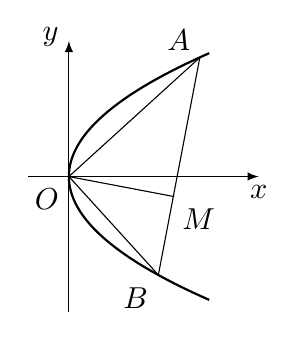
\begin{tikzpicture}[x=1pt, y=1pt,
    every node/.style={inner sep=0pt, font=\fontsize{10.5pt}{12.6pt}\selectfont}]
  \draw[line width=0.399pt] (-14.695,0) -- (64.989,0);
  \fill[line width=0.399pt] (68.576,0) .. controls (67.513,0.199) and (65.786,0.797) .. (64.591,1.494) -- (64.591,-1.494) .. controls (65.786,-0.797) and (67.513,-0.199) .. (68.576,0);
  \draw[line width=0.399pt] (0,-48.983) -- (0,45.396);
  \fill[line width=0.399pt] (0,48.983) .. controls (-0.199,47.92) and (-0.797,46.193) .. (-1.494,44.998) -- (1.494,44.998) .. controls (0.797,46.193) and (0.199,47.92) .. (0,48.983);
  % 三条割线。源内容流中 OB（路径 8）、OM（路径 9）以密集三次贝塞尔绘制，
  % 与直线最大偏差 0.0002 pt，此处按直线写出；O→A 另有路径 6（直线）与路径 10（贝塞尔）
  % 几何重合（偏差 < 0.01 pt），合并为一条。
  \draw[line width=0.399pt] (32.329,-35.562) -- (47.317,43.007);   % AB
  \draw[line width=0.399pt] (0,0) -- (47.317,43.007);              % OA
  \draw[line width=0.399pt] (0,0) -- (32.329,-35.562);             % OB
  \draw[line width=0.399pt] (0,0) -- (38.108,-7.269);              % OM
  % 抛物线 y^2 = 4px 的上、下两支（源路径 7 / 11，各 24 段三次贝塞尔）。
  % 拟合 x = 0.0255212 y^2（rms 0.0025 pt），即 4p = 39.177 pt。
  \draw[line width=0.797pt, domain=0:44.5724, samples=120, variable=\y]
    plot ({0.0255212*\y*\y}, \y);
  \draw[line width=0.797pt, domain=-44.5724:0, samples=120, variable=\y]
    plot ({0.0255212*\y*\y}, \y);

  \node[anchor=center] at (-6.647,50.369) {$y$};  % 源中心 (322.66,737.95)
  \node[anchor=center] at (39.683,49.329) {$A$};  % 源中心 (368.99,736.91)
  \node[anchor=center] at (68.573,-5.591) {$x$};  % 源中心 (397.88,681.99)
  \node[anchor=center] at (-7.997,-8.251) {$O$};  % 源中心 (321.31,679.33)
  \node[anchor=center] at (46.903,-15.521) {$M$};  % 源中心 (376.21,672.06)
  \node[anchor=center] at (24.123,-43.811) {$B$};  % 源中心 (353.43,643.77)
\end{tikzpicture}
%
% 【自验】
%   1) 探针编译：0 error、0 warning。
%   2) 600 dpi 双渲染差分量测标签净距：x 2.81、A 3.88、O 4.32、y 5.20、M 5.86、B 6.44 —— 最小 2.81 pt。
%   3) 线形：两轴与三条割线 0.399 pt；抛物线两支 0.797 pt，与源 w、d 值一致（全为实线）。
%   4) 抛物线拟合残差 rms 0.0025 pt；A、B 落在抛物线上（偏差 0.1 pt 内），OA⊥OB 斜率积 −1.000。
\end{center}
\nopagebreak[4]
\Needspace{4\baselineskip}
\textbf{解析}

设 $A\left(pt_1^2,\,2pt_1\right)$，$B\left(pt_2^2,\,2pt_2\right)$，其中 $t_1,t_2\ne0$（$A,B$ 不是原点）。

\Needspace{5\baselineskip}
\textbf{定值关系。} $OA\perp OB$：

\nopagebreak[4]
\[\overrightarrow{OA}\cdot\overrightarrow{OB}=p^2t_1^2t_2^2+4p^2t_1t_2=p^2t_1t_2(t_1t_2+4)=0 .\]

\Needspace{5\baselineskip}
因 $t_1t_2\ne0$，得

\nopagebreak[4]
\[t_1t_2=-4 .\]

\Needspace{5\baselineskip}
\textbf{弦 $AB$ 过定点。} 抛物线 $y^2=4px$ 上参数 $t_1,t_2$ 的弦方程为

\nopagebreak[4]
\[(t_1+t_2)y=2x+2p\,t_1t_2 .\]

（代入 $A$：左 $=(t_1+t_2)2pt_1$，右 $=2pt_1^2+2pt_1t_2$，相等。）将 $t_1t_2=-4$ 代入得 $(t_1+t_2)y=2x-8p$，令 $y=0$ 得 $x=4p$。故 $AB$ 恒过定点 $N(4p,0)$。

\Needspace{5\baselineskip}
\textbf{求轨迹。} 因 $OM\perp AB$ 且 $M\in AB$，$N\in AB$，故 $\angle OMN=90^\circ$，由泰勒斯定理 $M$ 在以 $ON$ 为直径的圆上：

\nopagebreak[4]
\[(x-0)(x-4p)+(y-0)(y-0)=0\ \Longrightarrow\ x^2+y^2-4px=0 .\]

\textbf{排除原点。} 若 $M=O$，则 $O\in AB$；但过 $O$ 的直线与抛物线除 $O$ 外至多还有一个公共点，不可能同时含 $A,B$，矛盾。故 $O$ 不在轨迹上。

\textbf{充分性。} 反之，过 $N(4p,0)$ 的任一直线（除 $x$ 轴）与抛物线交于两点 $A(t_1),B(t_2)$，由弦方程恒过 $N$ 反推 $8p+2pt_1t_2=0$，即 $t_1t_2=-4$，从而 $OA\perp OB$；自 $O$ 向该直线作垂线所得垂足即为 $M$，故圆上除 $O$ 外每一点都可取到。

综上，轨迹为圆 $x^2+y^2=4px$（$x\ne0$），即以 $(2p,0)$ 为圆心、$2p$ 为半径的圆，去掉原点。

验证：取 $p=1$，$t_1=1$、$t_2=-4$：$A(1,2)$，$B(16,-8)$，$\overrightarrow{OA}\cdot\overrightarrow{OB}=16-16=0$ ；$AB$ 为 $2x+3y=8$，过 $(4,0)$ ；垂足 $M\left(\dfrac{16}{13},\dfrac{24}{13}\right)$，$x^2+y^2=\dfrac{832}{169}$，$4px=\dfrac{64}{13}=\dfrac{832}{169}$ 。

\gkanswer{答案：轨迹方程为 $x^2+y^2-4px=0$（原点除外），即 $(x-2p)^2+y^2=(2p)^2$：以 $(2p,0)$ 为圆心、$2p$ 为半径的圆，去掉原点 $O$。}

\par\medskip

\end{answer}
\begin{answer}
\gksolhead{23}{}

\textbf{题目}：

某地区上年度电价为 $0.8$ 元/kW$\cdot$h，年用电量为 $a$ kW$\cdot$h　本年度计划将电价降到 $0.55$ 元/kW$\cdot$h 至 $0.75$ 元/kW$\cdot$h 之间，而用户期望电价为 $0.4$ 元/kW$\cdot$h　经测算，下调电价后新增的用电量与实际电价和用户期望电价的差成反比（比例系数为 $k$）．该地区电力的成本为 $0.3$ 元/kW$\cdot$h．

（1） 写出本年度电价下调后，电力部门的收益 $y$ 与实际电价 $x$ 的函数关系式；

（2） 设 $k = 0.2a$，当电价最低定为多少时仍可保证电力部门的收益比上年至少增长 $20\%$？

注：收益 = 实际用电量 ×（实际电价 $-$ 成本价）

\Needspace{4\baselineskip}
\textbf{解析}

\gksubpart{(1)}

\Needspace{5\baselineskip}
设实际电价为 $x$ 元/(kW·h)（$0.55\le x\le0.75$），则新增用电量 $=\dfrac{k}{x-0.4}$，实际用电量 $=a+\dfrac{k}{x-0.4}$。由「收益 = 实际用电量 ×（实际电价 $-$ 成本价）」，成本价 $0.3$，得

\nopagebreak[4]
\[y=\left(a+\frac{k}{x-0.4}\right)(x-0.3),\qquad 0.55\le x\le0.75 .\]

\gksubpart{(2)}

\Needspace{5\baselineskip}
上年收益 $=a(0.8-0.3)=0.5a$，要求 $y\ge1.2\times0.5a=0.6a$。取 $k=0.2a$：

\nopagebreak[4]
\[y=a\left(1+\frac{0.2}{x-0.4}\right)(x-0.3)=a\cdot\frac{(x-0.2)(x-0.3)}{x-0.4}.\]

\Needspace{5\baselineskip}
条件化为（$x-0.4>0$）

\nopagebreak[4]
\[(x-0.2)(x-0.3)\ge0.6(x-0.4)\]
\nopagebreak[4]
\[x^2-0.5x+0.06\ge0.6x-0.24\]
\nopagebreak[4]
\[x^2-1.1x+0.3\ge0\iff(x-0.5)(x-0.6)\ge0 .\]

在 $[0.55,0.75]$ 上解集为 $x\in[0.6,\,0.75]$。故电价最低定为 $0.6$ 元/(kW·h) 时，仍可保证收益比上年至少增长 $20\%$。

验证：$x=0.6$ 时用电量 $=a+\dfrac{0.2a}{0.2}=2a$，收益 $=2a\times0.3=0.6a$，恰为 $0.5a$ 的 $1.2$ 倍；$x=0.55$ 时收益 $=\left(a+\dfrac{0.2a}{0.15}\right)\times0.25=\dfrac{7a}{3}\times\dfrac14\approx0.583a<0.6a$，故 $0.6$ 确为最低值；$x=0.75$ 时收益 $\approx0.707a>0.6a$。

\gkanswer{答案（1）：$y=\left(a+\dfrac{k}{x-0.4}\right)(x-0.3)$，$0.55\le x\le0.75$}

\gkanswer{答案（2）：电价最低定为 $0.6$ 元/(kW·h)}

\par\medskip

\end{answer}
\begin{answer}
\gksolhead{24}{}

\textbf{题目}：

\Needspace{5\baselineskip}
已知函数

\nopagebreak[4]
\[f(x) = \begin{cases} f_1(x), & x \in \left[0, \dfrac{1}{2}\right), \\[4pt] f_2(x), & x \in \left[\dfrac{1}{2}, 1\right], \end{cases} \qquad \text{\text{其中} } f_1(x) = -2\left(x - \dfrac{1}{2}\right)^2 + 1,\]

\nopagebreak[4]
\[f_2(x) = -2x + 2.\]

（1） 在下面坐标系上画出 $y = f(x)$ 的图象；
\nopagebreak[4]
\begin{center}% f2000_spring_jingwan_science_q24_grid.tex — 2000 年·春季京皖卷·理科 第 24 题（空白平面直角坐标系，供作图）
%
% 【来源】`.work/phase4-b20/source/2000春季京皖理.pdf`
%   （SHA-256 37f07244497aa0a21be12d8a31eac78b61490f835f088719a5990463585a35ce），
%   第 2 页（印刷页 62）；qpdf --qdf 解包后对内容流逐路径解析。
% 【坐标口径】源 PDF 用户空间（原点左下、y 向上）。本图本地坐标
%   (x, y) = (x_page − 1062.162, y_page − 536.238)，1 单位 = 1 TeX pt；
%   O 取两轴交点；两轴等长（−15.874…75.784 pt），刻度 0.5 间隔 31.748 pt、1 间隔 63.497 pt。
% 【元素计数】8 条路径（x 轴／x 箭头／y 轴／y 箭头／4 条刻度线）＋ 7 个标签。
% 【标签】位置取 pdftotext -bbox 文本中心换算（源中心逐条记在 \node 行末）；
%   本图各标签按源中心放置，无微调。
\begin{tikzpicture}[x=1pt, y=1pt,
    every node/.style={inner sep=0pt, font=\fontsize{10.5pt}{12.6pt}\selectfont}]
  \draw[line width=0.399pt] (-15.874,0) -- (75.784,0);
  \fill[line width=0.399pt] (79.371,0) .. controls (78.308,0.199) and (76.581,0.797) .. (75.386,1.494) -- (75.386,-1.494) .. controls (76.581,-0.797) and (78.308,-0.199) .. (79.371,0);
  \draw[line width=0.399pt] (0,-15.874) -- (0,75.784);
  \fill[line width=0.399pt] (0,79.371) .. controls (-0.199,78.308) and (-0.797,76.581) .. (-1.494,75.386) -- (1.494,75.386) .. controls (0.797,76.581) and (0.199,78.308) .. (0,79.371);
  \draw[line width=0.399pt] (31.748,0) -- (31.748,3.175);
  \draw[line width=0.399pt] (0,31.748) -- (3.175,31.748);
  \draw[line width=0.399pt] (63.497,0) -- (63.497,3.175);
  \draw[line width=0.399pt] (0,63.497) -- (3.175,63.497);

  \node[anchor=center] at (-6.652,80.752) {$y$};  % 源中心 (1055.51,616.99)
  \node[anchor=center] at (-6.322,62.742) {$1$};  % 源中心 (1055.84,598.98)
  \node[anchor=center] at (-10.412,30.992) {$0.5$};  % 源中心 (1051.75,567.23)
  \node[anchor=center] at (-7.992,-8.248) {$O$};  % 源中心 (1054.17,527.99)
  \node[anchor=center] at (31.748,-7.838) {$0.5$};  % 源中心 (1093.91,528.40)
  \node[anchor=center] at (63.498,-7.838) {$1$};  % 源中心 (1125.66,528.40)
  \node[anchor=center] at (79.368,-5.598) {$x$};  % 源中心 (1141.53,530.64)
\end{tikzpicture}
%
% 【自验】
%   1) 探针编译：0 error、0 warning。
%   2) 600 dpi 双渲染差分量测标签净距：x 2.79，x 轴「0.5」「1」各 4.08，O 4.32，
%      y 轴「0.5」4.20、「1」4.44、「y」5.26 —— 最小 2.79 pt。
%   3) 线形：两轴与 4 条刻度线均 0.399 pt 实线；刻度长 3.175 pt，与源一致。
%   4) 刻度间距：x 轴 31.748/63.497 pt，y 轴 31.748/63.497 pt，两轴等长 91.658 pt。
\end{center}
\nopagebreak[4]
（2） 设 $y = f_2(x)$（$x \in \left[\dfrac{1}{2}, 1\right]$）的反函数为 $y = g(x)$，$a_1 = 1$，$a_2 = g(a_1)$，$\cdots$，$a_n = g(a_{n-1})$，求数列 $\{a_n\}$ 的通项公式，并求 $\lim\limits_{n \to \infty} a_n$；

（3） 若 $x_0 \in \left[0, \dfrac{1}{2}\right)$，$x_1 = f(x_0)$，$f(x_1) = x_0$，求 $x_0$．

\Needspace{4\baselineskip}
\textbf{解析}

\gksubpart{(1)}

当 $x\in\left[0,\tfrac12\right)$ 时 $f(x)=-2\left(x-\tfrac12\right)^2+1$：开口向下，顶点 $\left(\tfrac12,1\right)$，$f(1/2)=1$、$f(0)=\tfrac12$，在 $\left[0,\tfrac12\right)$ 上递增。当 $x\in\left[\tfrac12,1\right]$ 时 $f(x)=-2x+2$：由 $\left(\tfrac12,1\right)$ 递减到 $(1,0)$。两段在 $x=\tfrac12$ 处函数值都为 1，图象连续；最大值 1（$x=\tfrac12$），最小值 0（$x=1$）。作图时在给定坐标系中画出「左段抛物线弧 + 右段直线段」。

编者解答图（三个实心点分别为 $(0,\tfrac12)$、$(\tfrac12,1)$、$(1,0)$）：
\nopagebreak[4]
\begin{center}% 编者解答图，依据第24题分段函数绘制；不属于原卷题图。
\begin{tikzpicture}[x=4cm,y=4cm, every node/.style={font=\small}]
  \draw[->] (-.10,0)--(1.15,0) node[right] {$x$};
  \draw[->] (0,-.10)--(0,1.15) node[above] {$y$};
  \node[below left] at (0,0) {$O$};
  \foreach \t in {0.5,1} {
    \draw (\t,0)--(\t,.025) node[below=3pt] {$\t$};
    \draw (0,\t)--(.025,\t) node[left=3pt] {$\t$};
  }
  \draw[dashed,thin] (.5,0)--(.5,1)--(0,1);
  \draw[thick,domain=0:.5,samples=61] plot (\x,{-2*(\x-.5)^2+1});
  \draw[thick] (.5,1)--(1,0);
  \foreach \point in {(0,.5),(.5,1),(1,0)} \fill \point circle[radius=1.2pt];
\end{tikzpicture}
\end{center}
\nopagebreak[4]
\gksubpart{(2)}

\Needspace{5\baselineskip}
$f_2(x)=-2x+2$ 在 $\left[\tfrac12,1\right]$ 上单调递减，值域为 $[0,1]$，故其反函数

\nopagebreak[4]
\[g(x)=1-\frac x2,\qquad x\in[0,1] .\]

\Needspace{5\baselineskip}
于是 $a_1=1$，$a_n=1-\dfrac{a_{n-1}}{2}$。令不动点 $\lambda=1-\dfrac\lambda2$ 得 $\lambda=\dfrac23$，则

\nopagebreak[4]
\[a_n-\frac23=-\frac12\left(a_{n-1}-\frac23\right)\ \Longrightarrow\ a_n-\frac23=\left(-\frac12\right)^{n-1}\left(a_1-\frac23\right)=\frac13\left(-\frac12\right)^{n-1}.\]

\Needspace{5\baselineskip}
故

\nopagebreak[4]
\[a_n=\frac23+\frac13\left(-\frac12\right)^{n-1},\qquad \lim_{n\to\infty}a_n=\frac23 .\]

\gksubpart{(3)}

\Needspace{5\baselineskip}
由 $x_0\in\left[0,\tfrac12\right)$ 得 $x_1=f(x_0)=-2\left(x_0-\tfrac12\right)^2+1\in\left[\tfrac12,1\right)$，故 $f(x_1)=f_2(x_1)=2-2x_1$。条件 $f(x_1)=x_0$ 即

\nopagebreak[4]
\[2-2x_1=x_0\ \Longrightarrow\ x_1=1-\frac{x_0}{2}.\]

\Needspace{5\baselineskip}
与 $x_1=1-2\left(x_0-\tfrac12\right)^2$ 联立：

\nopagebreak[4]
\[1-2\left(x_0-\frac12\right)^2=1-\frac{x_0}{2}\ \Longrightarrow\ 4\left(x_0-\frac12\right)^2=x_0\]
\nopagebreak[4]
\[4x_0^2-4x_0+1=x_0\ \Longrightarrow\ 4x_0^2-5x_0+1=0\ \Longrightarrow\ x_0=\frac14\ \text{\text{或}}\ x_0=1 .\]

由 $x_0\in\left[0,\tfrac12\right)$，取 $x_0=\dfrac14$。

验证：(2) $n=2$：$a_2=g(1)=\tfrac12$，通项给 $\tfrac23-\tfrac16=\tfrac12$ ；$n=3$：$a_3=g\left(\tfrac12\right)=\tfrac34$，通项给 $\tfrac23+\tfrac1{12}=\tfrac34$ 。(3) $x_0=\tfrac14$ 时 $x_1=1-2\cdot\tfrac1{16}=\tfrac78$，$f\left(\tfrac78\right)=2-\tfrac74=\tfrac14=x_0$ ；另一根 1 不在 $\left[0,\tfrac12\right)$ 内，舍去。

\gkanswer{答案（1）：见解析（左段抛物线弧＋右段直线段，最大值 1、最小值 0）}

\gkanswer{答案（2）：$a_n=\dfrac23+\dfrac13\left(-\dfrac12\right)^{n-1}$，$\lim\limits_{n\to\infty}a_n=\dfrac23$}

\gkanswer{答案（3）：$x_0=\dfrac14$}

\par\medskip

\end{answer}